\chapter{Neocortex development and evolution}
\label{chap:neocortex}

\section{Introduction}
At the turn of the twentieth century, Ludwig Edinger and others developed an evolutionary model of brain development and
coined the name ``neocortex'' for the evolutionarily newest structure, which forms the dorsal region of the telencephalon~\citep{Jarvis2005}.
While the evolutionary history proposed by Edinger is still debated, the six-layered neocortex first appears in the fossil
record in small mammals, and it is generally considered a mammalian-specific feature~\citep{Rakic2009}.  The neocortex is
connected to higher cognitive functions in humans~\citep{Lui2011}, and its defects contribute to human diseases, such as
autism and Alzheimers disease~\citep{Walsh2008, Wexler2011}.

Different cell populations reside in distinct layers in the developing neocortex.  Neural progenitors line the ventricle.
Differentiated neurons migrate away from the ventricular zone to more superficial layers~\citep{Molyneaux2007}.  Using
genetic methods, much progress has been made to identify and determine the regulatory relationships among the key transcription
factors that control neocortex development and layer identity~\citep{Leone2008}.  Yet, the target genes of the key transcription
factors and the genomic enhancers that mediate regulatory interactions remain largely uncharacterized.  A fuller understanding
of the regulatory network that underlies neocortex development holds promise to guide differentiation protocols necessary for
stem cell therapies for human cognitive diseases~\citep{Hansen2011}.

The traditional approach to identify regulatory elements upstream of a gene, termed enhancer bashing, is to dissect the
regulatory domain around a gene into progressively smaller fragments until a sufficiently local region is identified~\citep{Luo2008}.
Enhancer bashing is an incremental approach for any gene, but it is particularly difficult for transcription factors, which
tend to reside in ``gene deserts'' and thus have huge regulatory domains~\citep{McLean2010, Ovcharenko2005}.  A superior technique
was recently developed to identify enhancers genome-wide using chromatin immunoprecipitation with the enhancer-associated
co-activator protein p300 and high throughput sequencing (p300 ChIP-seq)~\citep{Visel2009}.  The approach has been applied
\textit{in vivo} to identify candidate enhancers in the forebrain, midbrain, limb, and heart~\citep{Blow2010, May2012, Visel2009}.
Mouse transgenic assays show that around 80\% of candidates function as tissue-specific enhancers \textit{in vivo}~\citep{Visel2009}.
Here, we use p300 ChIP-seq to characterize the enhancer repertoire of the E14.5 mouse neocortex.  We analyze the expression patterns
and biological functions of the enhancer target genes.  We perform mouse transgenic enhancer assays to characterize the specificity
of ten candidates.  We compare the neocortex enhancers to enhancers from other tissues to further analyze tissue-specificity.  We then
examine the evolutionary conservation of the enhancers and use a zebrafish transgenic enhancer assay to evaluate the function of
neocortex enhancers in a vertebrate that lacks a neocortex.  Lastly, we demonstrate how pairing p300 ChIP-seq identification of
active enhancers with computational transcription factor binding site prediction offers a high-throughput, general technique to
derive local regulatory sub-networks that underlie tissue-specific development and maintenance.

\section{Results}

\begin{figure}[htbp]
\centering
\begin{tabular}{l}
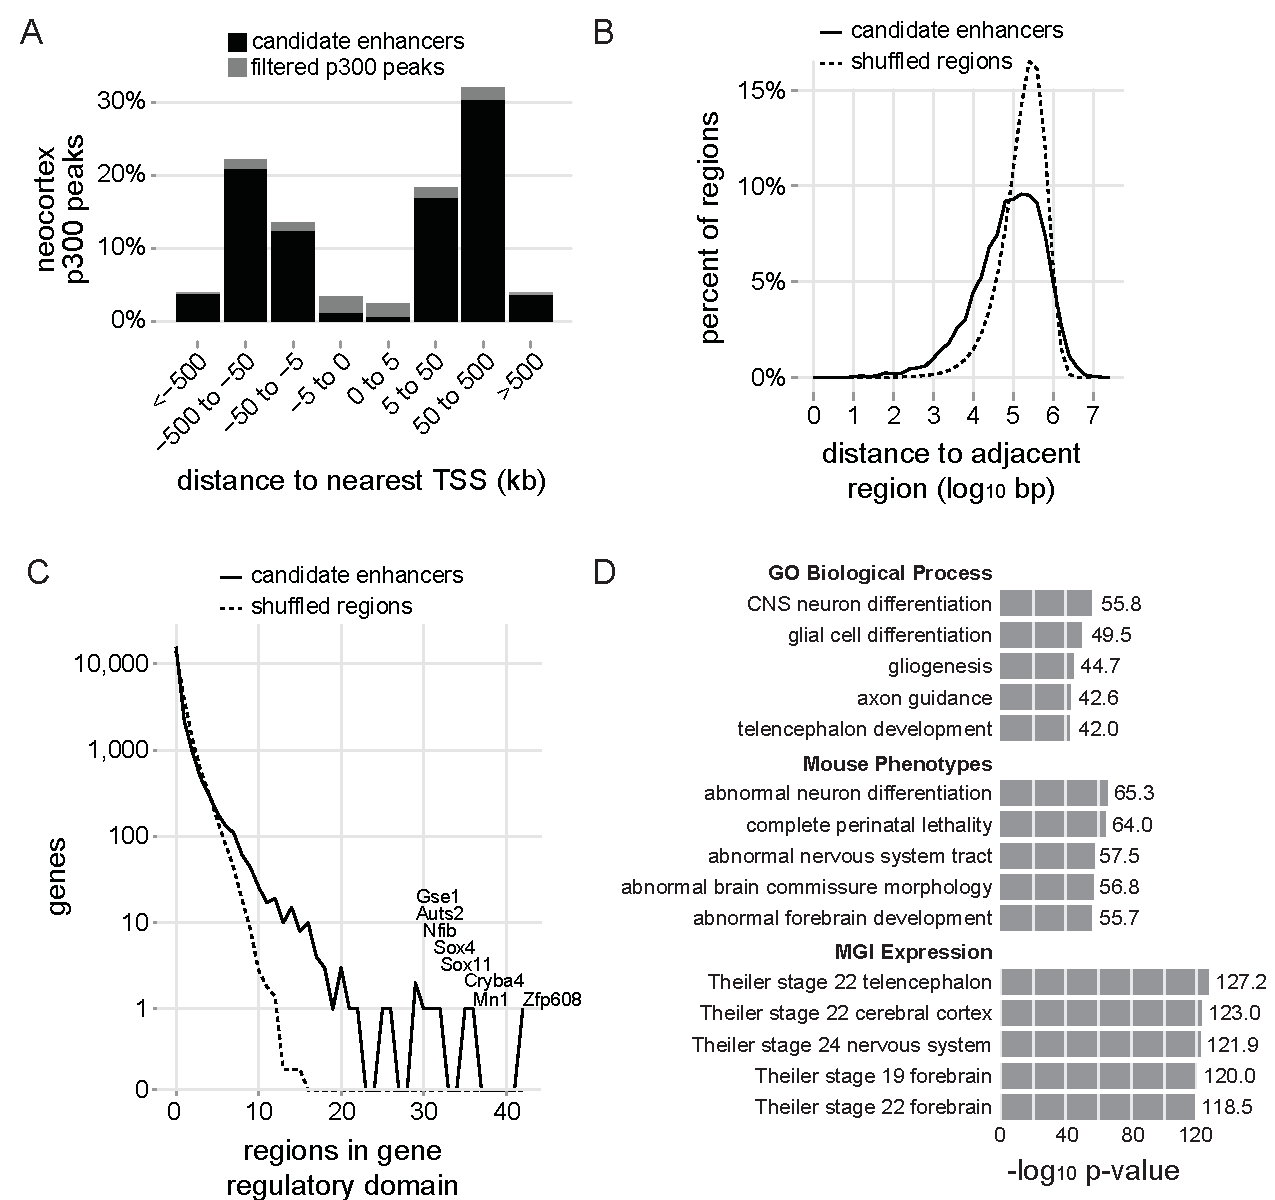
\epsfig{file=figures/ncxFigure1.pdf,width=0.99\linewidth,clip=,trim=0 0 0 0} \\
\end{tabular}
\caption[ChIP-seq for p300 identifies 6,629 candidate E14.5 neocortex enhancers]{
{\bf ChIP-seq for p300 identifies 6,629 candidate E14.5 neocortex enhancers.}
{\bf (A)} Distance from the p300 peaks to the nearest target gene.  Most peaks are
over 50kb from the nearest gene.  The ``filtered p300 peaks'' are removed for further
analysis due to overlap with repeat annotation or proximity to gene transcription start sites.  
{\bf (B)} Distance between adjacent candidate enhancers.  The enhancers show homotypic
clustering, tending to bunch more than randomly shuffled regions at distances from 1kb to 100kb.
{\bf (C)} Number of candidate enhancers in the regulatory domain of a gene.  Some genes
exhibit a high ``fan-in'' beyond that observed with a control of shuffled regions.
{\bf (D)} Top 5 terms per ontology of GREAT enrichments for the candidate neocortex
enhancers (``p-value'' is the region-based binomial p-value).  The candidates are
enriched near genes expressed in the neocortex and important for neocortex development.
}
\label{fig:ncxFig1}
\end{figure}

\subsection{ChIP-seq for p300 identifies candidate E14.5 neocortex enhancers}
To identify enhancers active in the developing mouse neocortex, we dissected the dorsal cortex from E14.5 mouse embryos and
performed chromatin immunoprecipitation followed by high-throughput sequencing (ChIP-seq) with an antibody to the
enhancer-associated p300 co-activator complex.  ChIP-seq identified 6,629 distal p300 binding sites ($>$ 2.5kb
from the nearest transcription start site), which are candidate neocortex enhancers (see Methods in \ref{sec:ncxMethods}).

As seen with other sets of tissue-specific developmental enhancers, the majority of the candidate neocortex enhancers are located
far from the nearest gene.  4,324 of the 6,629 candidate enhancers (65\%) are more than 50kb from the nearest transcription start site,
and 559 (8\%) are more than 500kb away (\figref{fig:ncxFig1}A) (see Methods in \ref{sec:ncxMethods}).  The candidate enhancers tend to cluster together
in the genome, and are enriched for occurring within 1 kb (fold: 4.0, p-value $< 10^{-45}$), 10kb
(fold: 4.7, p-value $< 10^{-280}$), and 100kb (fold: 2.0, p-value $< 10^{-360}$) of each
other (\figref{fig:ncxFig1}B) (see Methods in \ref{sec:ncxMethods}).  In other tissues, we have observed that large clusters of candidate enhancers associate
with genes known to be important to development of the tissue (data not shown); thus, a high ``fan-in'' is a signature
of a potentially critical gene.  For neocortex, large clusters neighbor both genes known to be critical for neocortex development
(e.g. \textit{Nfib} with 30 nearby peaks)~\citep{Piper2009} and potentially novel important genes (e.g. \textit{Zfp608} with 42 nearby peaks)
(\figref{fig:ncxFig1}C) (see Methods in \ref{sec:ncxMethods}).

\subsection{Candidate enhancers associate with genes expressed in the neocortex and important to neocortex development}
We used the Genomic Regions Enrichment of Annotations Tool (GREAT)~\citep{McLean2010} to evaluate the biological functions
of our 6,629 candidate neocortex enhancers.  GREAT assigns each gene a regulatory domain, associates each candidate enhancer
with the genes in whose regulatory domain it lies, applies the annotations of the genes to the enhancer, and performs a
statistical enrichment test.

The top Gene Ontology Biological Process enrichments for the candidate neocortex enhancers include gliogenesis
(300 enhancers; p-value: $1.8\times10^{-45}$), axon guidance (418 enhancers; p-value: $2.7\times10^{-43}$),
and telencephalon development (397 enhancers; p-value: $1.0\times10^{-42}$), all processes that occur in the E14.5
neocortex~\citep{Choi1988, Molyneaux2007}.  According to the Mouse Phenotypes ontology, our neocortex enhancers are enriched in the
regulatory domains of genes whose knockout or mutation results in abnormal forebrain development (419 enhancers; p-value: $1.9\times10^{-56}$)
and abnormal brain commissure development (396 enhancers; p-value: $1.7\times10^{-57}$) (\figref{fig:ncxFig1}D) (see Methods in \ref{sec:ncxMethods}).

Looking at gene expression, our candidate neocortex enhancers are enriched in the regulatory domain of genes expressed in the
cerebral cortex at Theiler Stage 22 (1,811 enhancers; p-value: $9.5\times10^{-124}$), which corresponds
approximately to the assayed tissue and timepoint~\citep{Kaufman1992}  (\figref{fig:ncxFig1}D).  A recent RNA-seq analysis
of microdissected E14.5 cerebral cortex identified genes expressed specifically in cortical layers~\citep{Ayoub2011}.  Our 6,629 candidate
enhancers are enriched for regulating genes specifically expressed in all three major layers: ventricular zone
(126 enhancers; p-value: $1.1\times10^{-25}$), subventricular zone (101 enhancers; p-value: $8.8\times10^{-25}$),
and cortical plate (251 enhancers; p-value: $1.8\times10^{-18}$) (see Methods in \ref{sec:ncxMethods}).  In total, the GREAT analysis shows
that the candidate enhancers regulate a wide variety of processes active across layers in the E14.5 neocortex.

\begin{figure}[htbp]
\centering
\begin{tabular}{l}
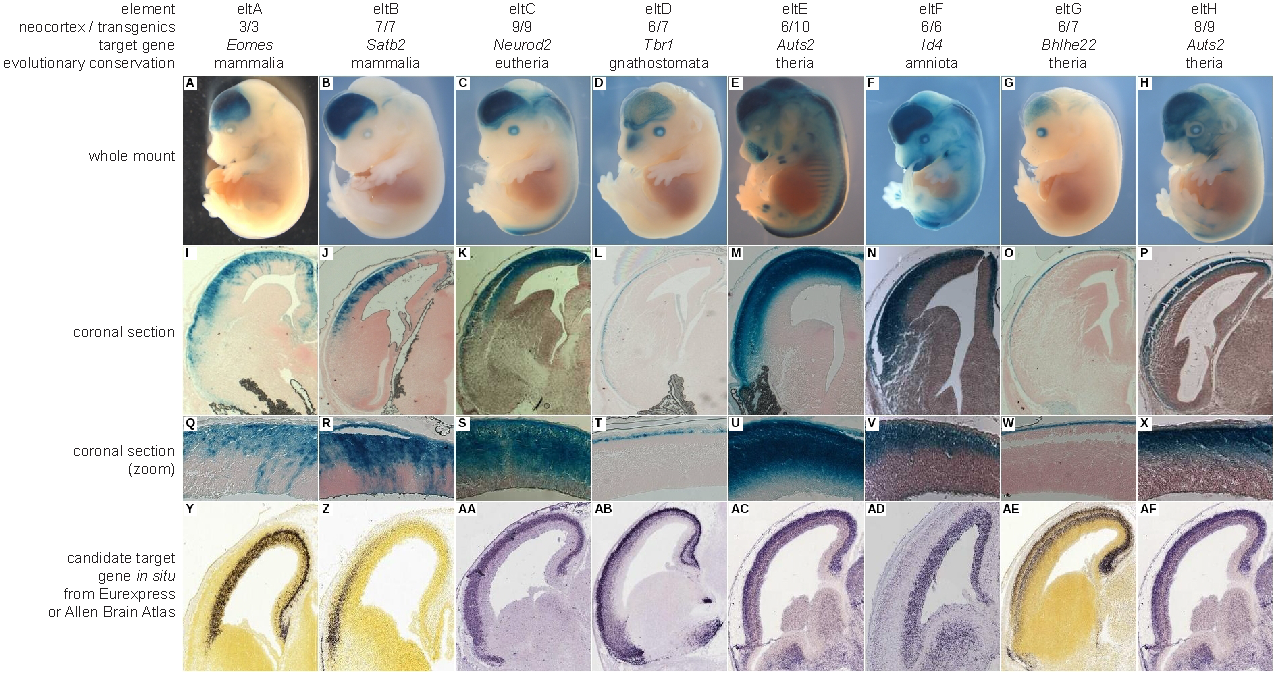
\epsfig{file=figures/ncxFigure2.pdf,width=0.99\linewidth,clip=,trim=0 0 0 0} \\
\end{tabular}
\caption[Candidate E14.5 neocortex enhancers drive lacZ reporter gene expression specifically
in the neocortex in mouse transgenic enhancer assays]{
{\bf Candidate E14.5 neocortex enhancers drive lacZ reporter gene expression specifically in the
neocortex in mouse transgenic enhancer assays.} We prioritized 10 candidates with a target gene
known to be important to neocortex development.  Of the 10 assayed candidates, 8 drive
reproducible expression in the neocortex.
{\bf (A-H)} Whole mounts show expression in the cerebral cortex.
{\bf (I-P)} Coronal sections reveal dorsal-specific expression exclusive of the ganglionic eminences.
{\bf (Q-X)} Zooms of coronal sections reveal distinct laminar patterns.
{\bf (Y-AF)} In situ of the candidate target gene at E14.5; coronal: Y-Z,
saggital: AA-AF.  Y,Z,AE from Allen Brain Atlas; AA-AD,AF from Eurexpress.
}
\label{fig:ncxFig2}
\end{figure}

\subsection{Candidate enhancers drive gene expression in distinct patterns in the E14.5 neocortex}
To demonstrate that the regions identified by ChIP-seq function as enhancers in the neocortex and to explore the tissue and
layer restriction of enhancer activity, we examined ten candidates in a transgenic mouse enhancer assay.  To select ten from the
set of 6,629 candidates, we prioritized elements with a putative target gene known to be an important neocortex transcription factor
or developmental gene: \textit{Auts2}, \textit{Bcl11b}, \textit{Bhlhe22}, \textit{Eomes}, \textit{Id4}, \textit{Neurod2}, \textit{Satb2}, and \textit{Tbr1}.  Eight of the ten assayed candidates drive
reproducible expression in the cerebral cortex visible in a whole mount (\figref{fig:ncxFig2}2A-H).

To explore the variety of specific expression patterns of the tested enhancers, we performed coronal sections of the transgenic
embryos (see Methods in \ref{sec:ncxMethods}).  Sections reveal that the assayed enhancers drive dorsal-specific expression in the neocortex exclusive of
the ganglionic eminences of the ventral telencephalon (\figref{fig:ncxFig2}I-P).  Sections also reveal laminar restriction of enhancer
activity.  Two enhancers -- eltD and eltG -- drive expression in a very superficial domain characterized by the Reelin protein.  The
other six enhancers are active primarily in the cortical plate.  None drive apparent activity in the progenitors of the ventricular
zone (\figref{fig:ncxFig2}Q-X).  For six of the eight positive enhancers, the domain of activity of the enhancer corresponds to a
domain of expression of the putative target gene~\citep{Science2009}.  Two enhancers -- eltA and eltF -- drive expression in the
cortical plate though the putative target genes (\textit{Eomes}/\textit{Tbr2} and \textit{Id4}) are restricted to the subventricular and ventricular zones,
respectively (\figref{fig:ncxFig2}Y-AF).  The lack of observed lacZ activity in the progenitor zones and the mismatch between observed
lacZ and the target gene \textit{in situs} could be due to a delay between mRNA expression and protein production.

\subsection{In vitro transfection of dissociated cortical neurons acts as a high throughput system that approximates enhancer activity in the neocortex}
The transgenic mouse reporter assay is an excellent system to examine \textit{in vivo} enhancer activity and tissue specificity, but it is
limited in throughput and does not readily lend itself to biochemical manipulation, such as ectopic expression or knockdown of a
putative regulator.  Such manipulations are much easier with an in vitro system.  We examined the activity of the ten candidates
in one such \textit{in vitro} system: transfection into acutely dissociated neurons from E14.5 dorsal cortex (see Methods in \ref{sec:ncxMethods}).

All enhancers that were active \textit{in vitro} also were active \textit{in vivo}, indicating that the \textit{in vitro} system is an
effective screen to identify \textit{in vivo} neocortex enhancers.  Five of the eight transgenic positive candidates are also positive
\textit{in vitro}, while the other three fail to drive activity significantly above background levels (\figref{fig:ncxFigS1}).
The two candidates that fail to drive reporter activity in the transgenic mouse also are inactive \textit{in vitro} (\figref{fig:ncxFigS1}).
None of seven selected negative control elements are active in the transfection system (\figref{fig:ncxFigS1}).  Transfection offers
a high-throughput system tenable to functional dissection of enhancers and upstream regulators.

\begin{figure}[htbp]
\centering
\begin{tabular}{l}
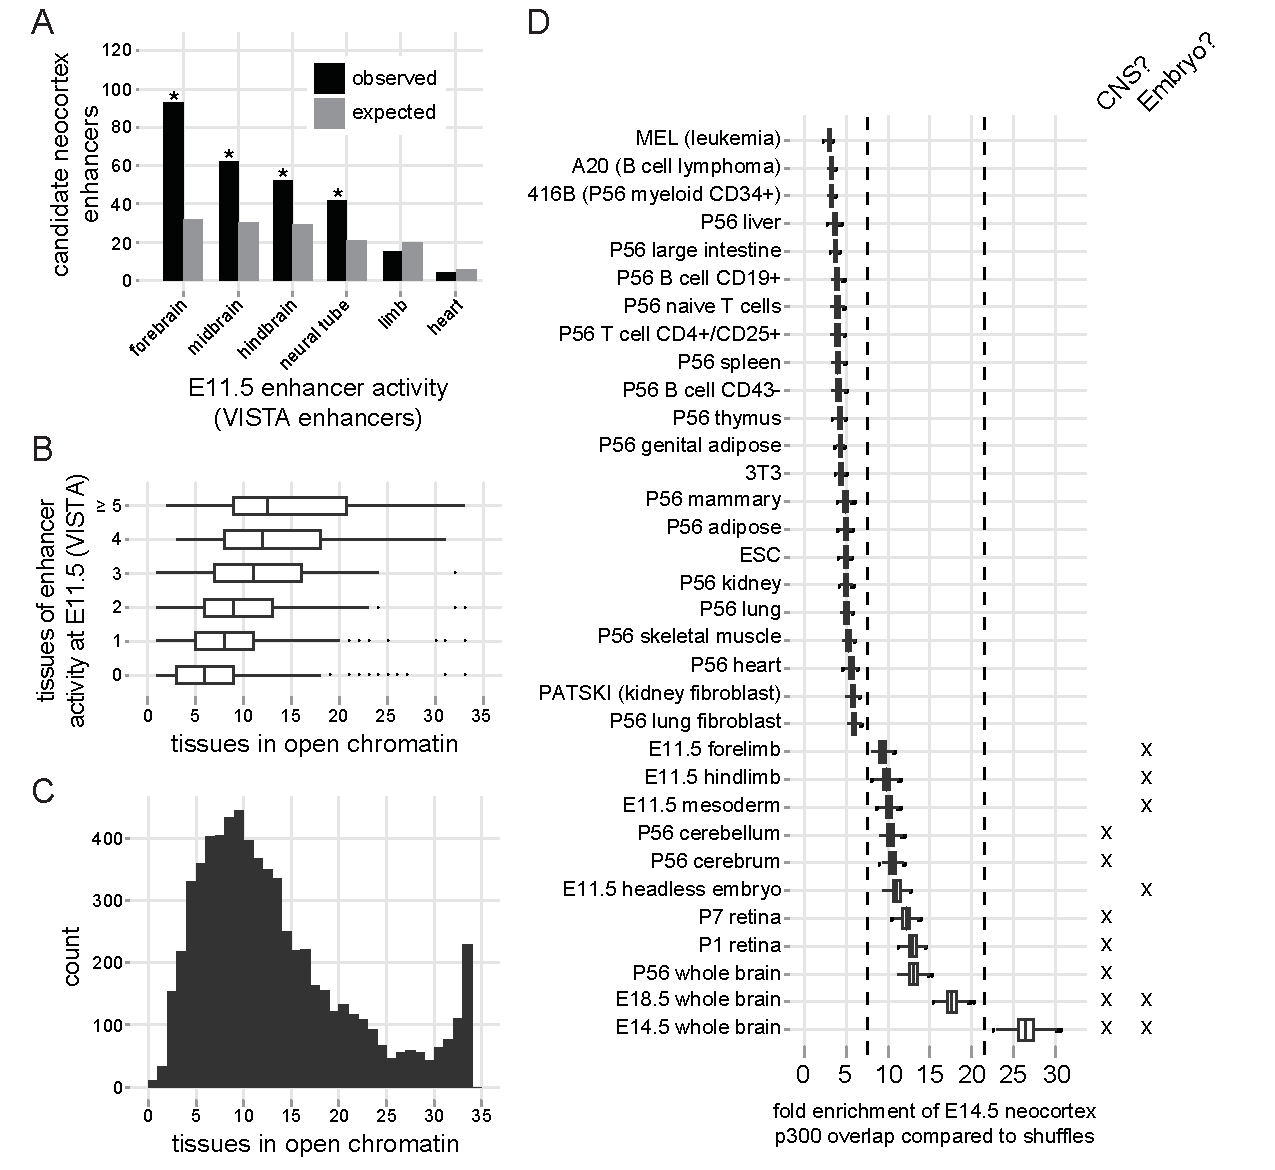
\epsfig{file=figures/ncxFigure3.pdf,width=0.99\linewidth,clip=,trim=0 0 0 0} \\
\end{tabular}
\caption[Candidate E14.5 neocortex enhancers are common to similar tissues and timepoints]{
{\bf Candidate E14.5 neocortex enhancers are common to similar tissues and timepoints.}
{\bf (A)} The VISTA Enhancer Browser includes E11.5 mouse transgenic enhancer assays for 214
neocortex candidates.  The enhancers drive activity in the central nervous system, most
specifically in the forebrain (* denotes enrichment p-value $< 10^{-5}$).
{\bf (B)} Distributions of the number of tissues in open chromatin (identified by DNAse I
hypersensitivity for 33 mouse tissues and cell lines) for 1,188 E11.5 VISTA enhancers of
varying tissue specificity.  More broadly active enhancers tend to overlap open chromatin
from more tissues.
{\bf (C)} Distribution of the number of tissues in which each of 6,629 candidate enhancers
overlaps an open chromatin region.  Most enhancers show tissue-restriction (few tissues),
but others are nearly constitutive (many tissues).  
{\bf (D)} Correlation of the candidate enhancers with open chromatin from various tissues.
For each tissue, the overlap of the candidate enhancers was compared to a control of randomly
shuffled regions, and the shuffling was repeated 1,000 times to define a distribution.  The
dotted lines show the only two clean separations of the observed distributions.  Embryonic
and central nervous system tissues show stronger overlap than other tissues.
}
\label{fig:ncxFig3}
\end{figure}

\subsection{Many candidate enhancers are common to similar tissues and timepoints}
Enhancers generally are considered to be tissue-specific, but some enhancers are active in multiple tissues~\citep{Heintzman2009}.
To measure the tissue-specificity of our E14.5 neocortex candidate enhancers, we examined overlap with previously tested enhancers
and DNAse I hypersensitivity open chromatin from a range of tissues and cell lines, which highlights active genes and regulatory
elements genome-wide~\citep{John2011}.

The VISTA Enhancer Browser~\citep{Pennacchio2006} includes results for E11.5 mouse transgenic enhancer assays for candidate human
DNA sequences.  The 1,188 tested regions that map to the mouse genome overlap 214 candidate E14.5 neocortex enhancers.  The tested
candidates are highly enriched for forebrain activity (93 = 43\%; fold: 2.9, p-value: $2.3\times10^{-31}$), but
some drive reproducible activity in the midbrain (62 = 29\%; fold: 2.0, p-value: $2.3\times10^{-10}$),
hindbrain (52 = 24\%; fold: 1.8, p-value: $1.5\times10^{-6}$), neural tube (42 = 20\%; fold: 2.0;
p-value: $6.3\times10^{-7}$), limb (15 = 7\%; fold: 0.75; p-value: $0.93$), or heart
(4 = 1.9\%; fold: 0.72; p-value: $0.84$) (\figref{fig:ncxFig3}A).  Thus, while many candidate neocortex enhancers
drive activity primarily in the expected tissue (forebrain), some are active in other contexts.

Across the full set of VISTA enhancers, the number of tissues in which an enhancer reproducibly drives activity correlates with
the number of tissues and cell lines in which it is resides in open chromatin (Fig. 3B).  Enhancers active in a single tissue at E11.5
are open chromatin in a median of 8 of the 33 examined tissues and cell lines.  Enhancers active in 5 or more E11.5 tissues are open
chromatin in a median of 13 contexts.  Thus, the number of tissues in which an enhancer is open chromatin is a proxy for the specificity
of the enhancer.

Of our 6,629 candidate neocortex enhancers, 2,789 (42\%) are open chromatin in fewer than 10 examined contexts, while 248 (3.7\%) are open
in all 33 examined tissues and cell lines (\figref{fig:ncxFig3}C).  Extrapolating from the correlation of open chromatin and specificity
for the VISTA enhancers, this suggests that activity of many of our candidate enhancers is restricted to the neocortex.  At the other
end of the spectrum, constitutive, distal open chromatin has previously been observed to be associated with \textit{Ctcf} binding sites~\citep{Heintzman2009}.
Of the 248 ``constitutive'' neocortex candidate enhancers, 212 overlap a known \textit{Ctcf} bound region.  This suggests that, in addition to many
neocortex-restricted enhancers, the 6,629 candidate neocortex enhancers include general enhancer elements and perhaps non-enhancer elements
such as \textit{Ctcf} insulators.

\subsection{Candidate enhancers correlate with open chromatin from neural and developmental contexts}
To examine trends in which tissues the candidate neocortex enhancers are open chromatin, we considered overlap on a per tissue basis.
As a control, we randomly shuffled the E14.5 neocortex candidate enhancers in the genome (1,000 times) and compared the basepair overlap
of the shuffled and original sets (see Methods in \ref{sec:ncxMethods}).  The E14.5 candidate enhancers overlap most significantly with tissues that match in
space (central nervous system, CNS) or time (embryonic development).  The strongest overlap is with open chromatin from whole brain at
the same E14.5 timepoint (z-score=19; median fold enrichment=26.5).  The separation of CNS or embryo tissues from other tissues is clear.
The worst fold enrichment against a shuffle for a CNS or embryo tissue (8.0 for one shuffle with E11.5 forelimb) is stronger than the best
observed overlap for other tissues (7.1 with P56 lung fibroblast) (\figref{fig:ncxFig3}D).  This comparison illustrates that tissue-specific
enhancers are more likely to be active in spatially or temporally matched contexts than in unrelated contexts.

\begin{figure}[htbp]
\centering
\begin{tabular}{l}
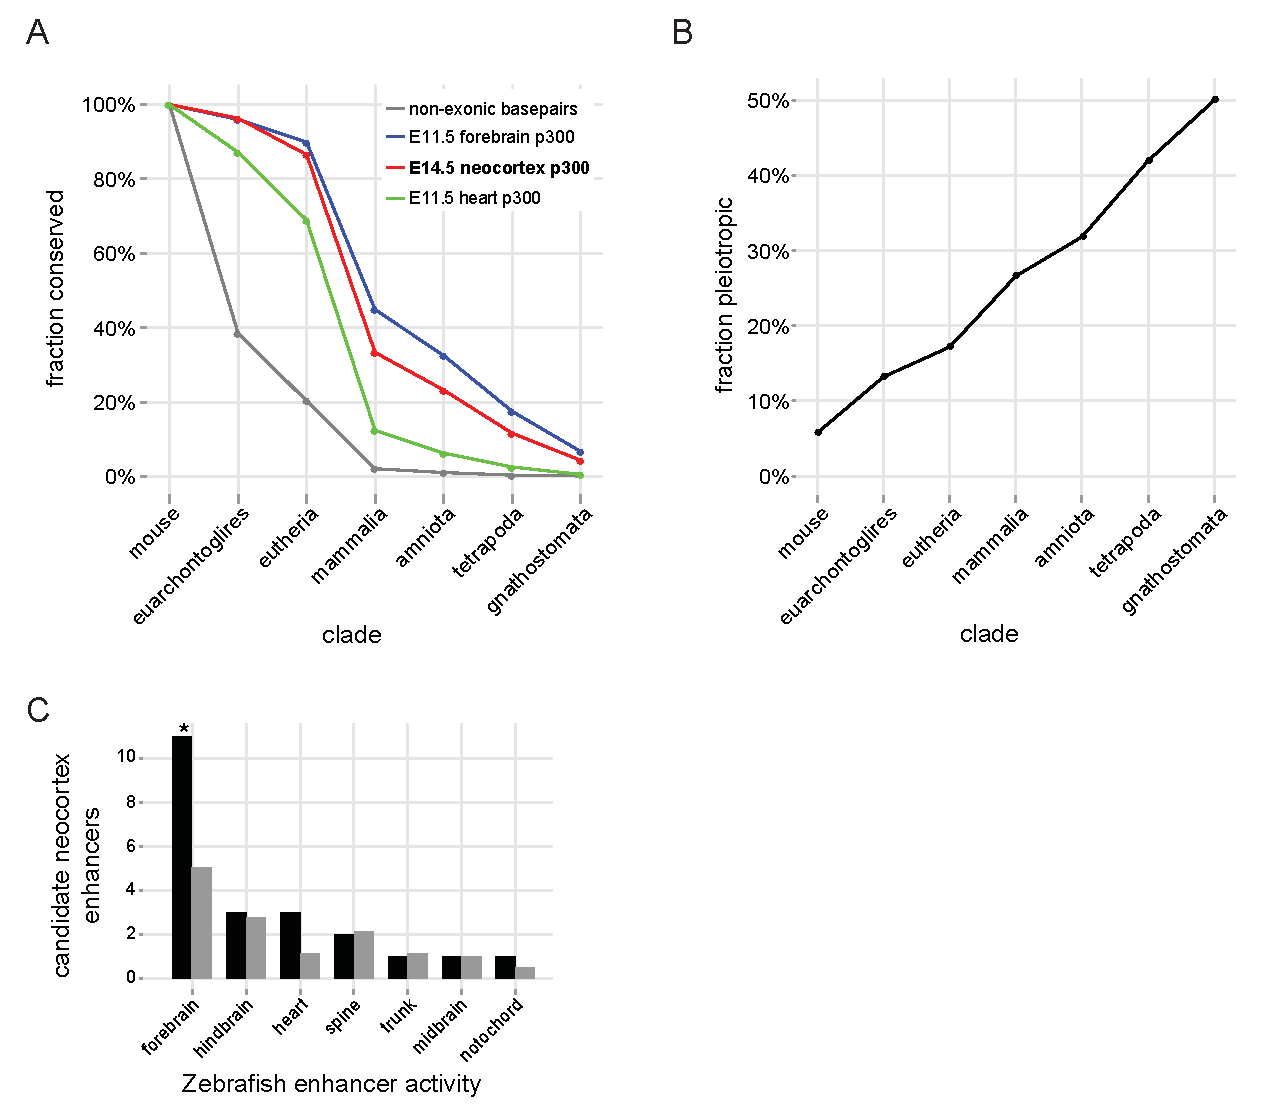
\epsfig{file=figures/ncxFigure4.pdf,width=0.99\linewidth,clip=,trim=0 0 0 0} \\
\end{tabular}
\caption[Evolutionary origins of neocortex enhancers]{
{\bf Evolutionary origins of neocortex enhancers.}
{\bf (A)} Evolutionary conservation of candidate regulatory elements.  Many candidate
neocortex enhancers pre-date the innovation of the six-layered neocortex in mammals.
{\bf (B)} Relationship between pleiotropy of candidate neocortex enhancers and evolutionary
conservation.  An enhancer is considered pleiotropic if it overlaps with candidate enhancers
from other tissues, specifically p300 peaks from E11.5 forebrain, midbrain, limb, and heart.
More ancient enhancers tend to be more pleiotropic.
{\bf (C)} The zebrafish cneBrowser includes transgenic enhancer assays for 21 of our
neocortex candidate enhancers (orthologous zebrafish DNA sequence).  The enhancers drive
activity in the zebrafish forebrain (* denotes enrichment p-value $< 0.05$).  
}
\label{fig:ncxFig4}
\end{figure}

\subsection{Most neocortex enhancers are evolutionary conserved, many beyond the mammalian ancestor}
The six-layered neocortex evolved in the ancestor of mammals~\citep{Rakic2009}, but many of the key genes that control its development, such
as \textit{Pax6} and \textit{Tbr1} are considerably more ancient, with some dating to well before the vertebrate ancestor.  We examined the conservation of our
6,629 candidate neocortex enhancers to trace the origins and evolution of neocortex regulatory elements.

The majority (4,278; 65\%) of the candidate neocortex enhancers exhibit signatures of evolutionary constraint (PhastCons score $>$ 350).  Very few
neocortex enhancers appear specific to the mouse lineage, as over 95\% (6,317) are conserved to human.  Over 86\% (5,737) are common to all
eutherian (placental) mammals.  Many candidate enhancers (1,543; 23\%) pre-date the innovation of the neocortex in mammals, and 289 (4\%) are
conserved to fish (gnathostomata) (\figref{fig:ncxFig4}A).  Just as ancient genes pattern the novel organ, so do ancient enhancers.

To examine how the conservation of candidate enhancers for an evolutionarily young organ compares to that of other organs, we analyzed
candidate enhancers from E11.5 heart and forebrain~\citep{Blow2010}.  Neocortex enhancers tend to be evolutionarily slightly
younger than forebrain enhancers and significantly older than heart enhancers and the
general genome (\figref{fig:ncxFig4}A).  Thus, enhancers for the evolutionary young neocortex are not markedly younger than enhancers
for more ancient structures.

\subsection{Ancient enhancers tend to be more pleiotropic}
While many enhancers are modular, others are pleiotropic and have multiple domains of activity.  We considered a candidate neocortex
enhancer to be pleiotropic if it overlaps a candidate enhancer from another tissue (using p300 peak sets for E11.5 heart, limb,
forebrain, and midbrain)~\citep{Blow2010} (see Methods in \ref{sec:ncxMethods}).  Only 6\% (14/229) of mouse-specific candidate enhancers are pleiotropic, while 50\%
(135/270) of fish-conserved candidate enhancers are.  Across evolutionary clades, more ancient enhancers tend to be more pleiotropic (\figref{fig:ncxFig4}B).

\subsection{Mouse neocortex enhancers drive expression in the zebrafish forebrain}
The surprising number of neocortex candidate enhancers that pre-date the mammalian innovation of the six-layered neocortex suggests
that the enhancers respond to a conserved regulatory signal, perhaps one used to pattern the general telencephalon in the
vertebrate ancestor.  We examined a zebrafish transgenic enhancer assay to investigate this hypothesis. A large zebrafish enhancer
screen~\citep{Li2010} assayed the zebrafish orthologs for 21 of our candidate neocortex enhancers, 11 of
which reproducibly drive reporter activity in the zebrafish forebrain (p-value: 0.002) (\figref{fig:ncxFig4}C).

\begin{figure}[htbp]
\centering
\begin{tabular}{l}
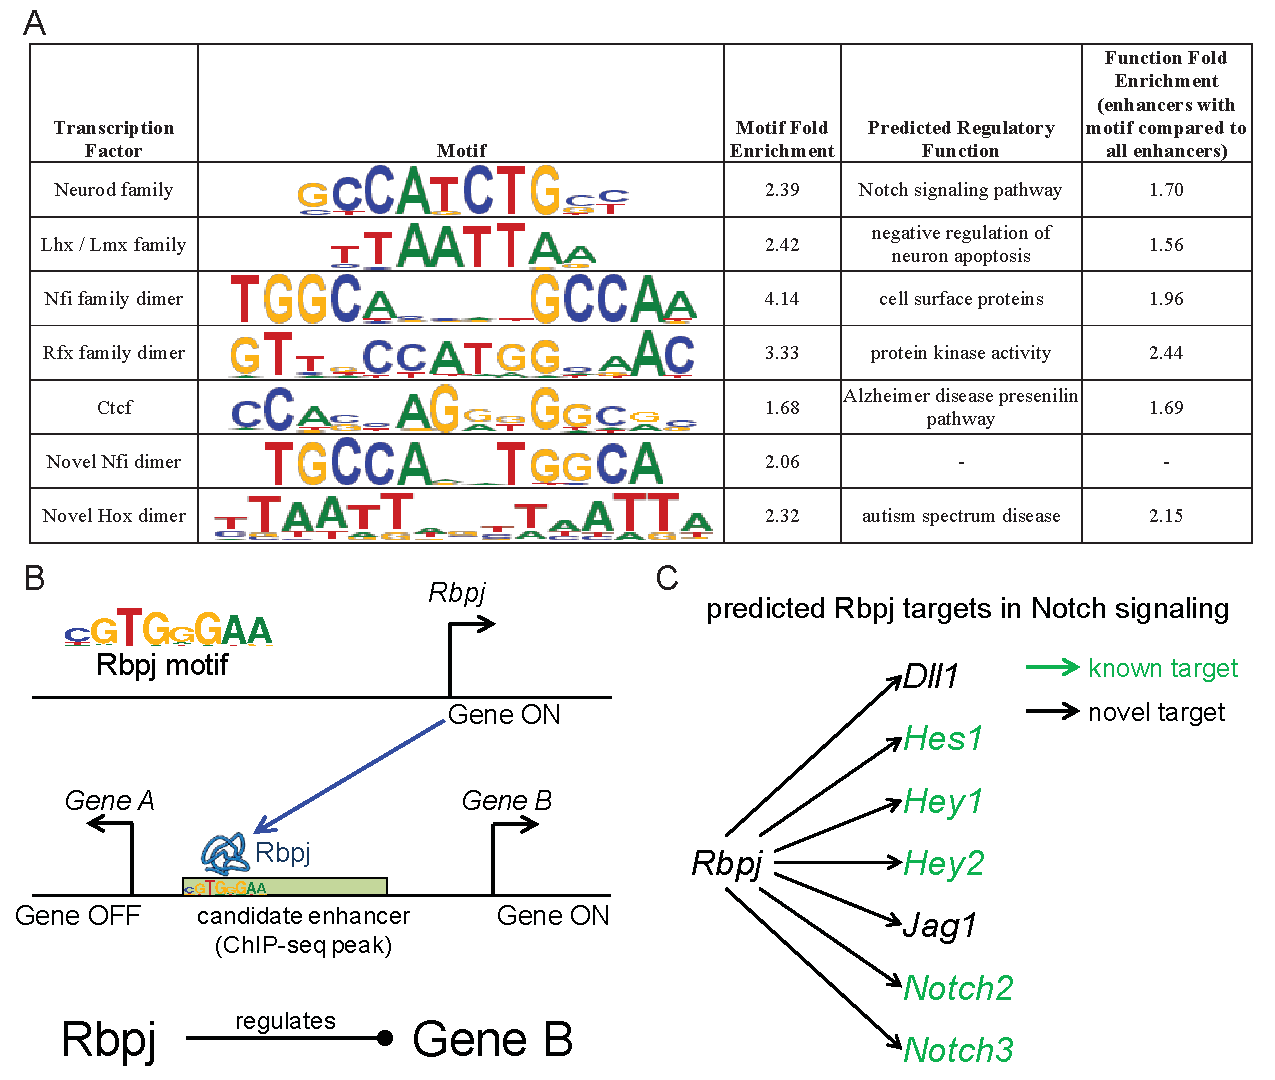
\epsfig{file=figures/ncxFigure5.pdf,width=0.99\linewidth,clip=,trim=0 0 0 0} \\
\end{tabular}
\caption[Binding site analysis reveals functional subsets and subnetworks]{
{\bf Binding site analysis reveals functional subsets and subnetworks.}
{\bf (A)} Motif discovery and motif enrichment analysis reveal known and novel
transcription factors that putatively regulate the candidate neocortex enhancers.
Motif fold enrichment is relative to [GC]-matched regions of the mouse genome.
Predicted regulatory function is the top relevant GREAT enrichment for the enhancers
with a motif hit compared to all candidate neocortex enhancers.
{\bf (B)} Binding site prediction in candidate enhancers suggests enhancer-mediated
gene interactions.
{\bf (C)} The predicted sub-network regulated by \textit{Rbpj} is enriched in Notch
signaling (p-value: $3.1\times10^{-4}$; fold: 4.8).
}
\label{fig:ncxFig5}
\end{figure}

\subsection{Enriched motifs are associated with functional subsets of neocortex enhancers}
To investigate the transcription factors that regulate our 6,629 candidate neocortex enhancers, we used a motif discovery and enrichment
analysis (see Methods in \ref{sec:ncxMethods}).  The analysis identifies a number of distinct enriched motifs, many for important regulators of neocortex development.
Compared to [GC]-matched regions from the mouse genome, the \textit{Neurod} (2,452 / 6,629 enhancers = 37\%; fold: 2.39), \textit{Lhx/Lmx} (2,129 = 32\%; fold: 2.42),
\textit{Nfi} (325 = 5\%; fold: 4.14), and \textit{Rfx} (195 = 3\%; fold: 3.33) family motifs are all highly enriched in the candidate neocortex enhancers.  Motif
discovery uncovered two novel enriched motifs for transcription factors known to be important in the neocortex, one an \textit{Nfi}
dimer (379 = 6\%; fold: 2.06) and the other a \textit{Hox} dimer (473 = 7\%; fold: 2.32).  Additionally, \textit{Ctcf} (652 = 10\%; fold: 1.68) -- which is well
known for its role as an insulator -- also is enriched (\figref{fig:ncxFig5}A).

Multiple biological processes occur across the E14.5 neocortex, including progenitor maintenance, neuron differentiation, and neuron
migration~\citep{Molyneaux2007}.  We hypothesized that our candidate neocortex enhancers encompass all of these processes, and that
enhancers involved in a specific function share a common motif.  To test this hypothesis, we used GREAT~\citep{McLean2010} to evaluate
the enrichments of the enhancers with a binding site for a given transcription factor (i.e. match to its motif) compared to the full set
of candidate enhancers (see Methods in \ref{sec:ncxMethods}).  GREAT predicts a number of cellular roles: the \textit{Neurod} family in Notch signaling (34 enhancers;
fold: 1.70; p-value: $9.0\times10^{-5}$), the \textit{Lhx/Lmx} family in negative regulation of neuron apoptosis
(44 enhancers; fold: 1.56; p-value: $3.4\times10^{-4}$), the \textit{Nfi} family in regulating cell surface proteins
(37 enhancers; fold: 1.96; p-value: $5.5\times10^{-5}$), and the \textit{Rfx} family in regulating protein kinase activity
(25 enhancers; fold: 2.44; p-value: $2.7\times10^{-5}$).  Intriguingly, it also predicts roles for transcription factors
and their target enhancers in neuronal diseases : Alzheimer disease presenilin pathway for \textit{Ctcf} (18 enhancers; fold: 1.69; p-value: $0.017$),
and autism spectrum disease for the \textit{Hox} family (33 enhancers; fold: 2.15; p-value: $1.9\times10^{-5}$) (\figref{fig:ncxFig5}A).

\subsection{Binding site analysis of candidate enhancers suggests regulatory networks}
\label{sec:ncxNetworks}
A true understanding of development requires knowledge of the enhancer-mediated transcription factor to target gene interactions that
comprise regulatory networks.  To start exploring the regulatory networks active in the E14.5 neocortex, we identified transcription
factor binding sites in the enhancer candidates.  As further support for individual binding site predictions, we required that the set
of enhancers predicted as bound by a given factor be enriched for a common functional role (\figref{fig:ncxFig5}B) (see Methods in \ref{sec:ncxMethods}).

As illustration of the concept of deriving a regulatory network from binding site predictions in candidate enhancers, we examined the
network centered around \textit{Rbpj}, with mediates Notch binding to DNA~\citep{Kopan2009}.  We predict conserved \textit{Rbpj} binding sites in 496
candidate neocortex enhancers at a p-value cutoff of 0.01.  The top biological pathway enriched for the predicted \textit{Rbpj} targets is Notch
signaling (p-value: $3.1\times10^{-4}$; fold: 4.8).  The combination of p300 ChIP-seq and binding site prediction
identifies \textit{Dll1}, \textit{Hes1}, \textit{Hey1}, \textit{Hey2}, \textit{Jag1}, \textit{Notch2}, and \textit{Notch3} as intriguing \textit{Rbpj} targets and highlights the enhancer regions that mediate
the predicted interaction.  A recent study identified five of these predicted target genes -- \textit{Hes1}, \textit{Hey1}, \textit{Hey2}, \textit{Notch2}, and \textit{Notch3} -- as
upregulated in neural stem cells that overexpress the Notch1 intercellular domain (N1ICD), which activates genes by binding to
\textit{Rbpj}~\citep{Li2012} (\figref{fig:ncxFig5}C).

\section{Methods}
\label{sec:ncxMethods}

\subsection{p300 ChIP-seq}
Embryonic neocortex tissue was dissected from E14.5 mouse embryos.  Cross-linking, chromatin isolation, and sonication were performed as
previously described~\citep{Barrera2008}.  Immunoprecipitation was performed with 4$\mu$g of anti-p300 antibody (Santa Cruz sc-585).

\subsection{ChIP-seq peak calling}
ChIP-seq reads were mapped to the mouse genome (mm9 assembly, NCBI MGSCv37) using ELAND, retaining only reads that map uniquely with 2 or
fewer mismatches.  Peaks were called using MACS~\citep{Zhang2008} with the p300 ChIP-seq reads as the treatment file, input DNA reads as
the control file, and the parameters ``\texttt{-{}-nomodel}, \texttt{-{}-shiftsize=100}, \texttt{-g mm}''.  Peaks overlapped by an exon, within 2.5kb of a transcription
start site, or covered over 50\% by annotated repeats were removed.  Exon and transcription start site annotation is from the UCSC knownGene
track (build 5)~\citep{Hsu2006}.  Repeat annotation is from the RepeatMasker track.

\subsection{Evaluating enhancer-to-gene and enhancer-to-enhancer distances}
To measure the distance from a candidate enhancer to the nearest gene, we used GREAT v2.0.0~\citep{McLean2010} with the ``single nearest'' association
rule, a maximum extension set to 10Mb, and no curated regulatory domains.

Homotypic clustering of the 6,629 candidate enhancers was compared to that of 6,629 random regions selected uniformly from the genome while avoiding
gaps, chrM, chrY, and random chromosomes.  The uniform selection was repeated 1,000 times to find the average number of elements that cluster in a
given window (1kb, 10kb, 100kb).  Significance of enrichment is calculated assuming a binomial distribution with the probability of success equal to
the average fraction of elements that cluster in a window across the 1,000 trials.

\subsection{Overlap with VISTA Enhancer Browser enhancers}
The VISTA Enhancer Browser~\citep{Pennacchio2006} includes results for mouse transgenic enhancer assays for candidate human DNA sequences.
We obtained 1,255 tested human sequences (downloaded Nov 10, 2011), and mapped the sequences to the mouse genome (mm9 assembly) using
liftOver (\texttt{-minMatch=0.8}) and lastz (\texttt{-{}-seed=match6}, \texttt{-{}-hsptresh=1800}, \texttt{-{}-gappedthresh=5000}, sequence identify $\ge$ 65\%, entropy $\ge$ 1.8).  We
successfully mapped 1,188 enhancers, including 176 forebrain enhancers and 343 enhancers active somewhere in the brain.  The tested sequences
overlap 214 of our candidate enhancers, with 93 active in the forebrain.  The significance of tested candidate neocortex enhancers driving
activity in the mouse forebrain is calculated using a hypergeometric enrichment test (forebrain: hyper[93 / 214; 176 / 1,188]).

\subsection{GREAT functional and expression enrichment analysis}
To evaluate functional and expression enrichments, we used GREAT v2.0.0~\citep{McLean2010} with the default association rule
(1kb+5kb basal domain with up to 1Mb extension and curated regulatory domains) and default significance thresholds (region-based binomial
fold = 2, region-based binomial FDR = 0.05, gene-based hypergeometric FDR = 0.05).  A lower region-based binomial fold criterion (= 1.6) was
used for the MGI Expression ontology.

We evaluated specific enrichment in the ventricular zone, subventricular zone, and cortical plate using a custom ontology based on a recent
RNA-seq dataset~\citep{Ayoub2011}.  We consider a gene to be specific to a layer if it has a layer RPKM (reads per kilobase of model)
$> 64$ and $> 2\times\mbox{(RPKM of the adjacent layer)}$ (average of adjacent layers for the subventricular zone).

\subsection{Mouse transient transgenic enhancer assay and sectioning}
The candidate enhancer sequences were PCR amplified from mouse genomic DNA (coordinates in \tabref{tab:ncxTableS1}) into an HSP68-lacZ reporter
vector.  The constructs were inserted into single cell FVB mouse embryo using pronuclear injection (Xenogen Biosciences / Taconic).  Embryos
were harvested at E14.5 and stained for lacZ expression.

\subsection{Cortical neuron transfection assay}
Neocortex tissue was dissected from E14.5 mouse embryos, and the neurons were acutely dissociated.  Enhancer constructs were transfected
into neurons using the Amaxa nucleofection system (Lonza)~\citep{Maasho2004}.

\subsection{Overlap with DNAse I hypersensitivity open chromatin data}
We used the UCSC Table Browser~\citep{Karolchik2004} to obtain open chromatin hotspots for 33 mouse tissues and cell lines produced
by the ENCODE Consortium~\citep{John2011, Myers2011}.  For tissues with multiple replicates, only basepairs
within hotspots in all replicates were retained (``basepair-wise AND'').

We used simulation to measure the significance of the overlap for our 6,629 candidate neocortex enhancers with open chromatin.  For each
tissue and cell line, we measured the number of basepairs of overlap between the open chromatin hotspots and: the 6,629 candidate
enhancers ($B_{ncx}$) and 6,629 random regions selected uniformly from the genome ($B_{shuffle}$).
The uniform selection was repeated 1,000 times to obtain a distribution of $B_{shuffle}$.  We calculate the fold enrichment
of the overlap for the candidate enhancers compared to the uniform selections ($fold = B_{ncx}/B_{shuffle}$), such that
a fold above (below) one indicates more (less) overlap for the candidate enhancers than for a random shuffle.

\subsection{Evolutionary conservation analysis}
We considered a candidate enhancer to be under purifying selection if it overlaps a region from the PhastCons Elements
track (phastConsElements30way) that scores at least 350~\citep{Siepel2005}.  We tagged candidates with depth of conservation based on
pairwise alignment nets from UCSC~\citep{Kent2003}.  We obtained all regions of the genome in the level 1 and 2 nets; eliminated large
duplications (genomicSuperDups)~\citep{Bailey2002}, pseudogenes (pseudoYale60), and known exons (knownGene:exon)~\citep{Hsu2006}; and considered
a basepair conserved to a given clade only if it is conserved to the previous clade.  Clades were represented by: euarchontoglires (human hg19,
chimp panTro3, rhesus rheMac2); boreoeutheria (horse equCab2, dog canFam2); eutheria (elephant loxAfr3); theria (opossum monDom5); mammalia
(platypus ornAna1); amniota (chicken galGal3, lizard anoCar2); tetrapoda (frog xenTro3); gnathostomata (tetraodon tetNig2, fugu fr2, zebrafish
danRer7, stickleback gasAcu1, medaka oryLat2); vertebrata (lamprey petMar1).  For clades with multiple representatives, a basepair is considered
conserved if it aligns to any of the representatives (two genomes required for gnathostomata).  A candidate enhancer is tagged with the deepest
clade to which at least 200bp of the candidate is conserved.

In \figref{fig:ncxFig4}A, ``non-exonic basepairs'' is all basepairs in the mouse genome not in large duplications, pseudogenes, exons, or gaps.

\subsection{Pleiotropy analysis}
A candidate neocortex enhancer is considered to be pleiotropic if it overlaps a candidate enhancer (i.e. p300 peak) from E11.5 forebrain,
midbrain, limb, or heart~\citep{Blow2010}.

\subsection{Overlap with zebrafish cneBrowser enhancers}
The zebrafish cneBrowser~\citep{Li2010, Persampieri2008} includes results for zebrafish transgenic enhancer assays for candidate zebrafish
DNA sequences.  We obtained 164 tested zebrafish sequences (downloaded Nov 10, 2011), and mapped the sequences to the mouse genome (mm9 assembly)
using lastz (\texttt{-{}-seed=match6}, \texttt{-{}-hsptresh=1800}, \texttt{-{}-gappedthresh=5000}, sequence identify $\ge$ 65\%, entropy $\ge$ 1.8).  We successfully mapped 129
enhancers (21 overlap a candidate neocortex enhancer), including 31 forebrain enhancers (11 overlap), and 44 enhancers active somewhere in the
brain (12 overlap).  The significance of tested candidate neocortex enhancers driving activity in the zebrafish forebrain is calculated
using a hypergeometric enrichment test (hyper[11 / 21; 31 / 129]).

\subsection{Motif discovery and enrichment analysis}
We compiled a library of 1,339 motifs (position weight matrices) that model the binding preferences for 646 transcription factors.  We predicted
binding sites using the motifs in the 6,629 candidate neocortex enhancers and in randomly selected [GC]-matched regions from the mouse genome at
a motif match threshold of 0.9~\citep{Kel2003}.  Motif fold enrichment is the number of candidate enhancers with a match to the motif divided
by the number of random regions with a motif match.

To predict biological functions for the subset of enhancers with a match for each enriched motif, we performed a GREAT foreground/background
test~\citep{McLean2010} with default association rules.  Significance criteria are:
fold $ > 1.5$, genes hit $ > 10$, FDR $ < 0.5$.

\subsection{Regulatory network analysis}
To build a regulatory network centered around \textit{Rbpj}, we predicted binding sites for \textit{Rbpj} in the candidate enhancers using the \textit{Rbpj} motif and a motif
match threshold of 0.9.  We evaluated the subset of enhancers with a match to the motif with GREAT v2.0.0~\citep{McLean2010} and selected the target
genes for the top enriched term in the Pathway Commons ontology.

\section{Discussion}
ChIP-seq for epigenomic enhancer marks enables genome-wide identification of candidate enhancers for an assayed tissue or cell line.
Here, in order to investigate the development and evolution of the neocortex, we use ChIP-seq for the co-activator p300 to identify 6,629 candidate
enhancers for the E14.5 mouse neocortex (\figref{fig:ncxFig1}A).

Development is a dynamic process with enhancers becoming active and inactive across space and time.   Through comparison to open chromatin
from other tissues, we demonstrate that the regulatory program of the E14.5 neocortex most closely resembles that of tissues that match in
either space (central nervous system) or time (embryonic development).  The correlation with space is stronger, and it illustrates that
pan-neural genes are accompanied by pan-neural enhancers.  The strong sharing during embryonic development (independent of space) suggests
a common developmental circuit, and GREAT analysis indicates a role for the shared enhancers in negative regulation of differentiation
(p-value: $3.1\times10^{-29}$; fold: 2.2).  This suggests three distinct classes of enhancers active in the developing
neocortex: pan-neural enhancers maintaining neural identity and driving differentiation, pan-developmental enhancers preventing differentiation,
and transient spatiotemporal-specific enhancers orchestrating the transition from dominance by the pan-developmental enhancers (undifferentiated)
to dominance by the pan-neural enhancers (differentiated).

Just as in development, but on a grander timescale, enhancers arise and fade across evolution.  Given that the six-layered neocortex is a
mammalian innovation, it might be expected that the genomic regions that drive neocortex development originated in the mammalian ancestor.
Most (86\%) candidate mouse neocortex enhancers are pan-eutherian, which implies that much of the regulatory circuitry was present in the
ancestor of placental mammals.  Surprisingly, many candidate enhancers (23\%) pre-date the mammalian ancestor and 289 (4\%) are conserved to fish.
These pre-mammalian enhancers were co-opted into a role in the mammalian-specific neocortex.

We hypothesized that the co-opted enhancers likely regulated genes in the general forebrain before gaining a specific role in the neocortex.
This hypothesis implies more generally that the signals and transcription factors that pattern the neocortex were modified from those that
patterned the ancient forebrain.  Eleven of 21 tested zebrafish orthologs of candidate mouse enhancers drive reporter activity in the zebrafish forebrain, demonstrating
that neocortex enhancers respond to deeply conserved signals for patterning the forebrain.  We expect that most organs, including recently evolved
ones, rely on ancient signals and enhancers to pattern their development.

While enhancers generally are regarded as tissue-restricted and modular, our analysis clearly shows that many enhancers are active in multiple
tissues and at multiple timepoints.  We observed that pleiotropic candidate enhancers -- those bound by p300 in multiple tissues -- exhibit
deeper evolutionary conservation.  There are two possible evolutionary histories for a pleiotropic enhancer.  First, the enhancer could have
had multiple functions since its origin, with the deeper conservation explained by greater constraint on the multifunctional element.
Second, the enhancer could have had a single ancestral role and later acquired additional ones.  The deeper conservation would then be explained
as a side effect of it being easier to add functionality to an existing enhancer than to create one de novo.  As the neocortex is a novel mammalian
structure, the latter is the more likely history for deeply conserved neocortex enhancers.  This recapitulates a general observation about ancient
enhancers, in which a core activating element is conserved and then supplemented in a clade-specific manner to serve multiple,
precise functions~\citep{Royo2011}.

ChIP-seq is a powerful, high-throughput tool to catalog the enhancers active in a tissue, but a simple enumeration does not explain how development
is regulated through the enhancers.  In contrast, genetic perturbation experiments, such as gene knockouts, identify gene to gene regulatory relationships
but are low-throughput and unable to identify the genomic enhancers that mediate regulatory interactions.  In fact, genetic perturbations can not
differentiate between direct and indirect genetic effects.  Here we illustrate how analysis of candidate enhancers with accurate computational transcription
factor binding site prediction provides a high-throughput tool to derive putative genetic regulatory networks of direct interactions.  We provide an example
using the motif for \textit{Rbpj} to identify 7 candidate target genes involved in Notch signaling.  When deployed en masse, this approach will generate an extensive
network of regulatory interactions active in any assayed tissue.  While ChIP-seq of every relevant transcription factor in every tissue is beyond the
current and conceivable reach of technology, computational analysis of ChIP-seq for a small number of enhancer associated marks could provide a rich
picture of developmental regulatory networks.  Knowledge of the regulatory networks will in turn inform our understanding of neocortex disease
and evolution.
